\begin{figure}[t]
    \center
    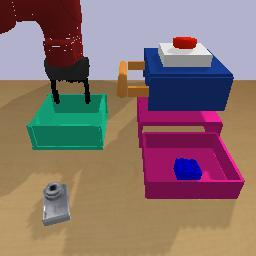
\includegraphics[height=0.24\linewidth]{val/imgs/views/simb_view.jpeg}
    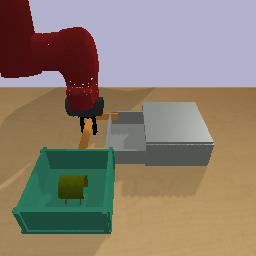
\includegraphics[width=0.24\linewidth]{val/imgs/views/sima_view1.jpeg}
    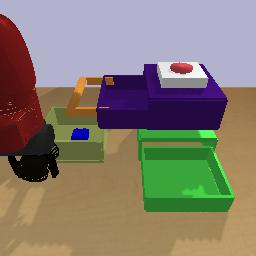
\includegraphics[height=0.24\linewidth]{val/imgs/views/sima_view2.jpeg}
    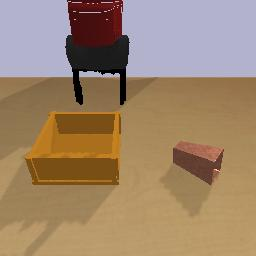
\includegraphics[width=0.24\linewidth]{val/imgs/views/sima_view3.jpeg}
    \caption{Randomly sampled scenes from our simulated multi-task environment. To practice in a sampled scene, the agent must infer the potential behaviors that the scene affords.}
    \label{fig:simenvs}
\end{figure}

\begin{figure}[t]
    \center
    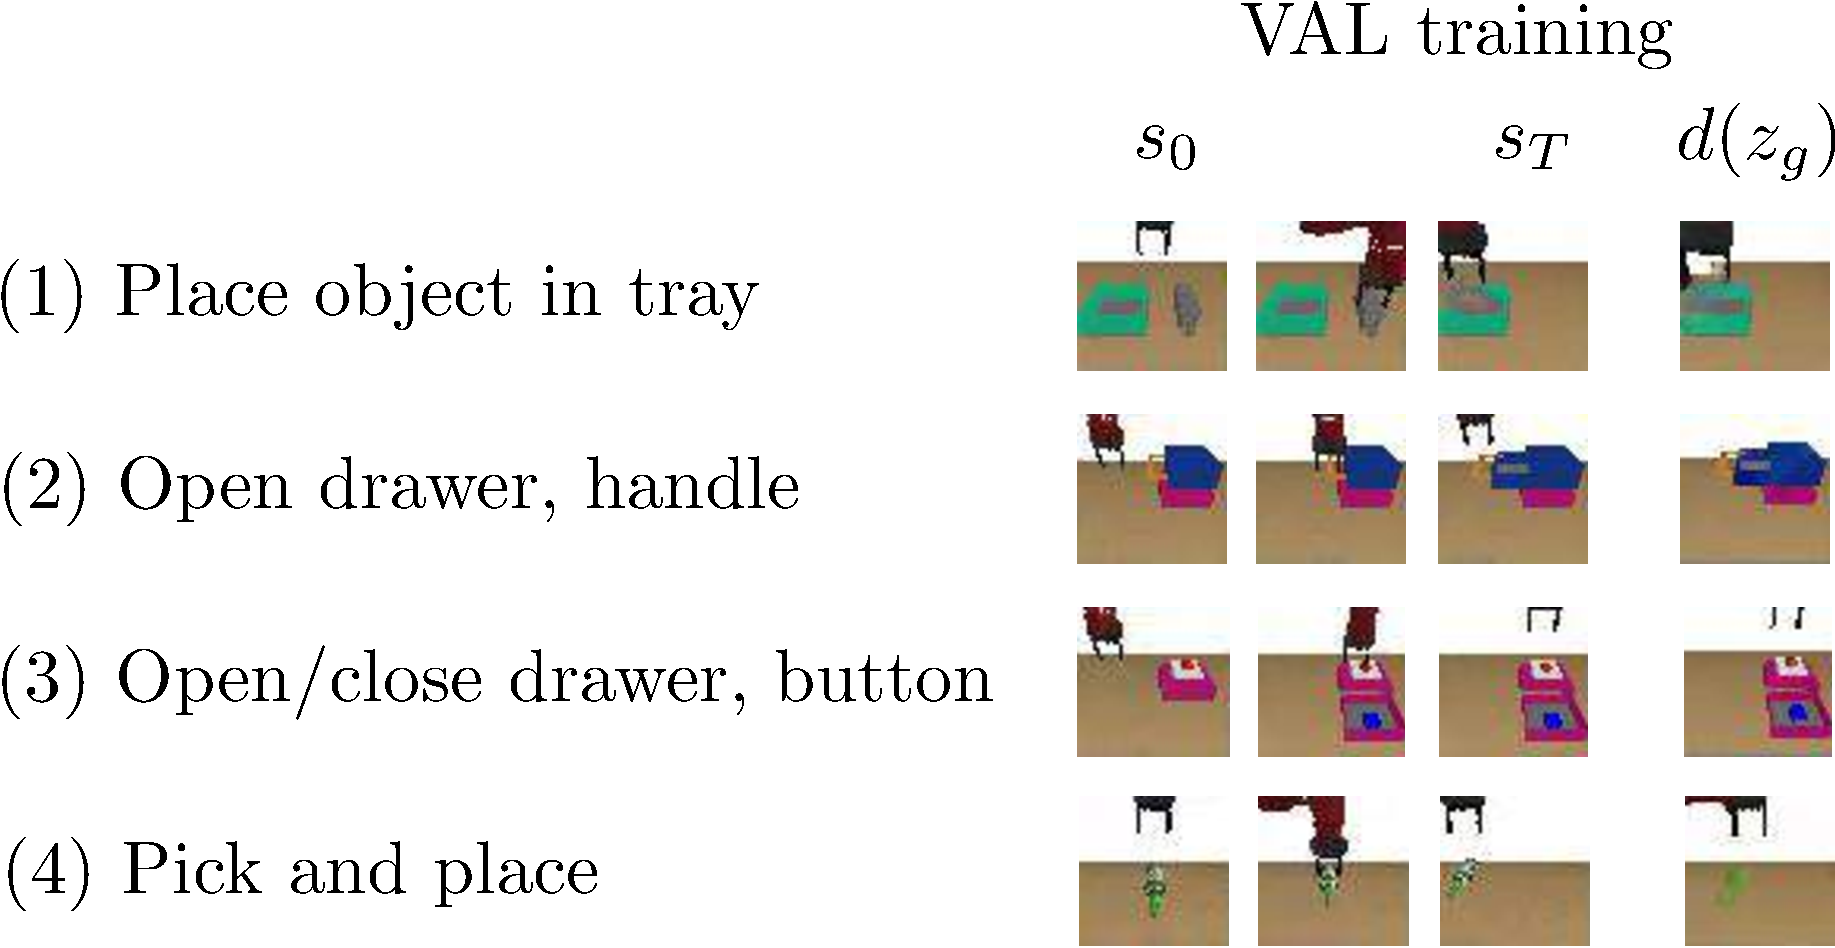
\includegraphics[width=0.6\linewidth]{val/imgs/fig_rollouts_sim-crop-compressed.pdf}
    \caption{Training rollouts from VAL. For each environment, the reconstruction of a sampled affordance is shown on the rightmost column, and frames from a trajectory attempting to achieve that affordance is shown on the left.}
    \label{fig:simenvs}
\end{figure}

\begin{figure}[t]
\centering
    \begin{subfigure}[b]{0.2\textwidth}
        \begin{flushright}
        
        Initial Image
        
        \vspace{0.35cm}
        
        CVQVAE (Ours)
        
        \vspace{0.35cm}
        
        CCVAE
        
        \vspace{0.35cm}
        
        CBiGAN
        
        \vspace{0.35cm}
        
        VAE
        
        \vspace{0.22cm}
        
        \end{flushright}
        
    \end{subfigure}
    \begin{subfigure}[b]{0.3\textwidth}
        \centering
        
        \scalebox{1.85}{
                \adjustbox{trim=0 16 0 0,clip} { 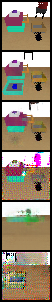
\includegraphics[width=0.1\textwidth]{val/imgs/samples/sim1/s1.png} } \hspace{-12px}
                \adjustbox{trim=0 16 0 0,clip} { 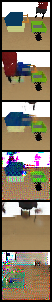
\includegraphics[width=0.1\textwidth]{val/imgs/samples/sim1/s2.png} } \hspace{-12px}
                \adjustbox{trim=0 16 0 0,clip} { 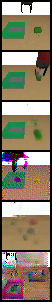
\includegraphics[width=0.1\textwidth]{val/imgs/samples/sim1/s3.png} } \hspace{-12px}
                \adjustbox{trim=0 16 0 0,clip} { 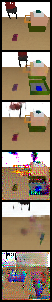
\includegraphics[width=0.1\textwidth]{val/imgs/samples/sim1/s5.png} } \hspace{-12px}
                \adjustbox{trim=0 16 0 0,clip} { 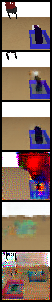
\includegraphics[width=0.1\textwidth]{val/imgs/samples/sim1/f1.png} } \hspace{-12px}
                \adjustbox{trim=0 16 0 0,clip} { 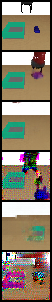
\includegraphics[width=0.1\textwidth]{val/imgs/samples/sim1/f2.png} } \hspace{-12px}
            }
    \end{subfigure}
    \caption{Samples on test environments in simulation. In each column, the top image is the conditioning image $s_0$ and the images below are conditionally sampled images. The left four columns are relatively successful samples for our affordance model, each showing the potential outcome of a behavior. The right two columns are failure modes, lacking diversity or altering an object's geometry or color. }
    \label{fig:samples}
    % \vspace{-0.5cm}
\end{figure}